\section[INTRODUCCI\'ON HIST\'ORICA DEL DODECAFONISMO]{INTRODUCCI\'ON HIST\'ORICA DEL DODECAFONISMO}\label{ch:historia}

\subsection{La historia de la disonancia}
La disonancia siempre ha formado parte de las experiencias musicales. Con la consonancia ha venido siempre emparejada la disonancia, mano a mano, para confrontarse y contrastarse mutuamente. Y es que sin una jam\'as podr\'ia existir la otra.

En la Antigua Grecia, la armon\'ia musical se consideraba unida al resto del universo. La rotaci\'on de los astros emit\'ia sonidos arm\'onicos, y era la armon\'ia la que apaciguaba el alma. ¿Pero qu\'e era la armon\'ia, sino la unión de consonancia y disonancia? Como dijo Arist\'oteles:
\begin{quote}
\emph{El alma es armon\'ia porque la armon\'ia es mezcla y s\'intesis de contrarios, y de contrarios se compone el cuerpo.}\footnote{J. de Aixquivel,
\textit{Memorias de Historia Antigua}, 1989.}
\end{quote}

Es bien sabido que la Escuela de Pit\'agoras, con su estudio sobre proporciones entre notas, buscaba encontrar cu\'ales eran los intervalos m\'as consonantes. Encontraban, a su vez, aquellos que no lo eran, y es as\'i como se dio comienzo a la teor\'ia de la disonancia. 

Ya en la Edad Media, la polifon\'ia fue forjando normas sobre el uso de las disonancias.
%Jam\'as se la apart\'o o se la rechaz\'o: era un elemento m\'as a utilizar. 
La primera regla compositiva de la m\'usica occidental\footnote{Knud Jeppesen, \textit{Counterpoint: the polyphonic vocal style of the sixteenth century},
1931.} fue la \emph{regla franconiana}, que expresaba que
las disonancias deb\'ian ocurrir en la parte d\'ebil del comp\'as, mientras que las consonancias en la parte fuerte. Es as\'i como los compositores trenzaban consonancia y disonancia al tejer los hilos de la m\'usica.

Poco a poco la disonancia pas\'o a ser usada como floritura mel\'odica: en notas de paso, apoyaturas o retardos, entre otras. Esta funci\'on mel\'odica fue impregnando el contrapunto hasta llegar a ser pieza clave en la continuidad de las voces. Adquiri\'o entonces una nueva funci\'on contrapunt\'istica, ¿y qui\'en no se ha emocionado al escuchar una disonancia \textit{bachiana}?

Pero la disonancia estaba a\'un inscrita a la tonalidad regente. No fue hasta la introducci\'on de acordes extra\~nos que la disonancia pas\'o a ser el centro de atenci\'on. Para ello hubo que esperar hasta el siglo XIX, que fue testigo de un desarrollo del sistema arm\'onico sin precedentes. 

\subsection{Wagner, Mahler y la emancipaci\'on de la disonancia}
Aunque las posibilidades que ofrec\'ia la tonalidad parec\'ian infinitas, sus l\'imites empezaron a entreverse hacia finales del siglo XIX. En palabras de Arnold Schoenberg: 
\begin{quote}
\emph{El o\'ido se fue familiarizando gradualmente con gran n\'umero de disonancias, hasta que lleg\'o a perder el miedo a su efecto perturbador.}\footnote{Arnold Schoenberg, \emph{Composition with twelve tones}, en \emph{Style and Idea}, 1950.}
\end{quote}

%El periodo de la historia de la m\'usica predominante en el siglo XIX, com\'unmente llamado Romanticismo, 
Esta \'epoca
culmin\'o con los dramas musicales de Richard Wagner, en los que todos los elementos de la obra estaban detalladamente estudiados por el compositor. A este concepto lo llamaba \emph{Gesamtkunstwerk} (<<{obra de arte total}>>\footnote{Richard Wagner, \emph{Oper und Drama}, 1851.}), ya que %cre\'ia poseer la responsabilidad de reunir todas las artes en una misma obra. Wagner 
se aseguraba personalmente de que en sus \'operas las artes esc\'enicas, musicales, po\'eticas y visuales se combinaran entre s\'i a la perfecci\'on.

\begin{figure}
\begin{center}
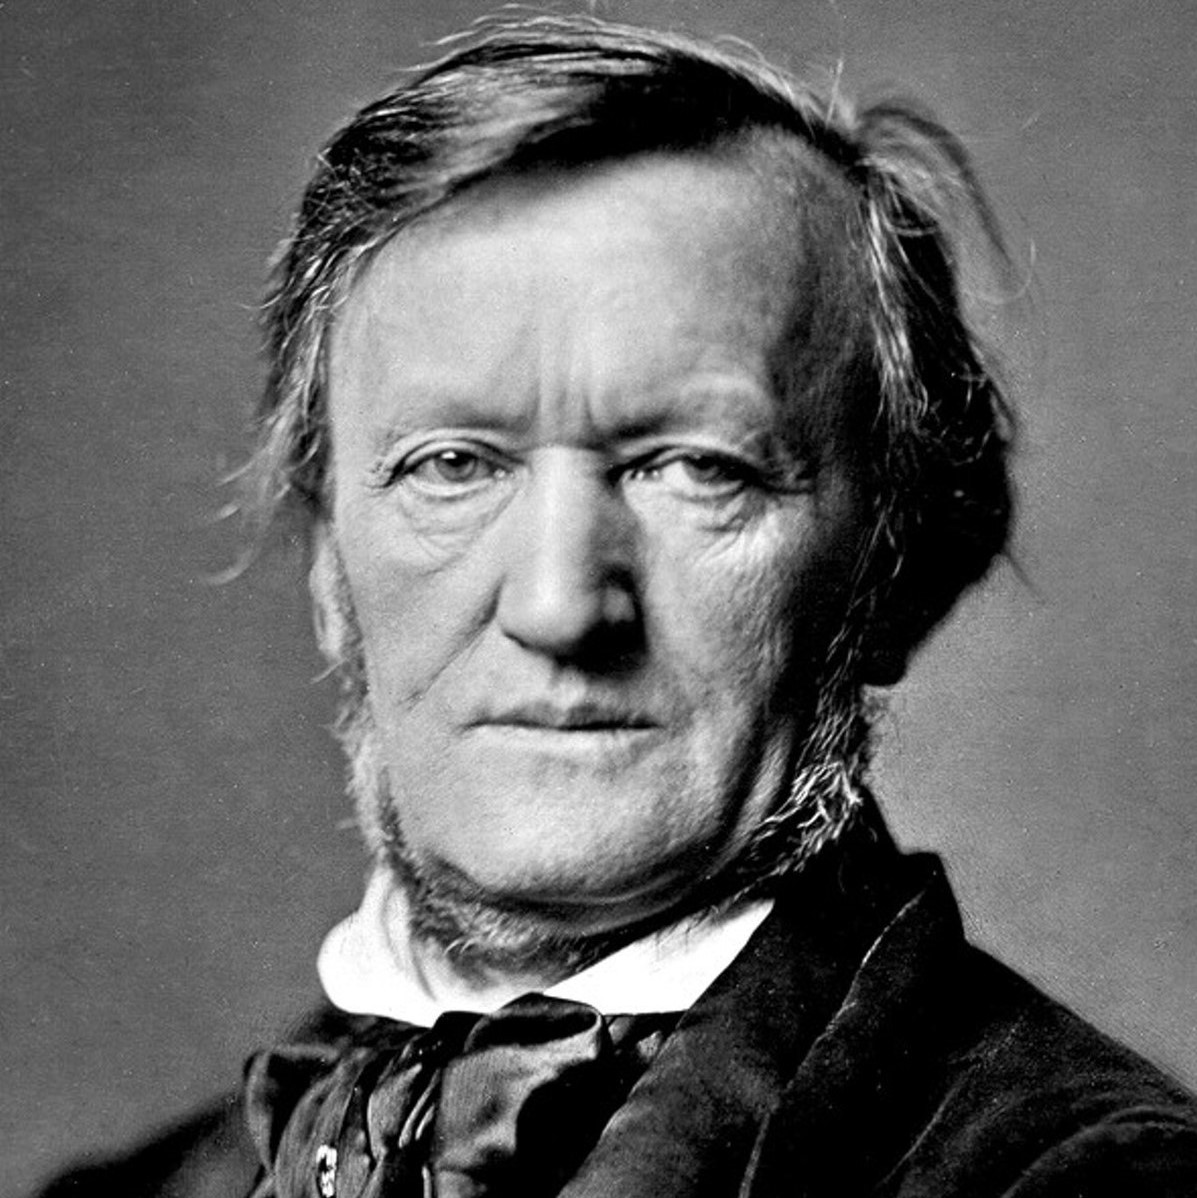
\includegraphics[width=3cm]{Richard_Wagner.jpg}\\
{Richard Wagner\\(1813--1883)}
\end{center}
\end{figure}

La idea del \emph{Gesamtkunstwerk} la desarroll\'o alrededor de 1850, y la plasm\'o en su totalidad en su ciclo de cuatro \'operas \href{https://www.youtube.com/watch?v=1PBhlPeTJ_g}{\textit{Der Ring des Nibelungen}}, estrenado el 16 de agosto de 1876. Wagner control\'o y cre\'o cada aspecto de la tetralog\'ia, desde la m\'usica hasta el libreto, el vestuario y la escenograf\'ia. Incluso mand\'o crear su propia sala de conciertos en Bayreuth, el \emph{Festspielhaus}, para que el escenario se adecuara a sus ideas sobre el pensamiento y la cultura musical.

As\'i, a ojos de compositores posteriores, se hab\'ian agotado todas las posibilidades de la m\'usica tonal, y quiz\'as ya hab\'ia comenzado el viraje hacia el predominio de la disonancia con su abundante uso del cromatismo, como en el famoso primer acorde del drama musical \href{https://www.youtube.com/watch?v=SF4zN-Okonc}{\textit{Tristan und Isolde}} (1865). %Consta de las notas Fa, Si, $\mbox{Re\#}$ y $\mbox{Sol\#}$, y sus intervalos desde el Fa son una cuarta aumentada, una sexta aumentada y una novena aumentada.

Despu\'es de Wagner, otros compositores tambi\'en previeron emancipar la disonancia en sus obras. Gustav Mahler reflejaba en sus sinfon\'ias la fragilidad de la tradici\'on anterior y la inminencia de su ruptura. Ya m\'as adelante, en 1911, utiliza en el \href{https://www.youtube.com/watch?v=vHyV8noUXC0}{Adagio} de su D\'ecima Sinfon\'ia una disonancia con casi todas las doce notas de la escala crom\'atica. Sin duda, la tonalidad quer\'ia ser reemplazada.

\begin{figure}
\begin{center}
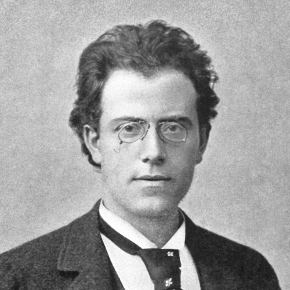
\includegraphics[width=3cm]{Gustav_Mahler.jpg}\\
{Gustav Mahler\\(1860--1911)}
\end{center}
\end{figure}

Siguiendo la concepci\'on del progreso como un camino ascendente, el paso siguiente para la composici\'on musical deb\'ia consistir en deshacerse progresivamente de la tonalidad y desarrollar la <<{emancipaci\'on de la disonancia}>>\footnotemark[3]. As\'i fue como Arnold Schoenberg ide\'o sus teor\'ias del pensamiento musical, y \'estas dieron paso a la creaci\'on de la atonalidad. \cite{kinney}

\subsection{Hacia el atonalismo de Schoenberg}
Fuertemente influido por Wagner y Mahler desde su adolescencia, Schoenberg comenz\'o componiendo al estilo posrom\'antico de su \'epoca, llevando el cromatismo y la orquestaci\'on hasta el extremo. Sin embargo, y no espont\'aneamente, empez\'o a buscar en sus composiciones que cada sonido tuviera valor por s\'i mismo, un valor independiente de su funcionalidad tonal.

\begin{figure}
\begin{center}
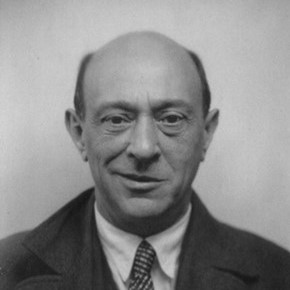
\includegraphics[width=3cm]{Arnold_Schoenberg.jpg}\\
{Arnold Schoenberg\\(1874--1951)}
\end{center}
\end{figure}
Para \'el, la m\'usica no estaba intr\'insecamente dirigida a una t\'onica. En las progresiones, lo importante era el paso de un acorde a otro, y no hacia d\'onde se dirig\'ian \'estos. Adem\'as, \'el opinaba que se deb\'ian poder utilizar las notas de los modos eclesi\'asticos libremente, por lo que consideraba las notas no diat\'onicas tan v\'alidas como las diat\'onicas. Esto hac\'ia imposible distinguir unas de otras, no pudiendo identificar apenas la t\'onica. De esta, y de otras muchas formas, Schoenberg consegu\'ia que la jerarqu\'ia tonal quedara desestabilizada. \cite{kinney}

De esta \'epoca es su primera obra importante, \href{https://www.youtube.com/watch?v=vqODySSxYpc}{\emph{Verkl\"arte Nacht}} (<<{Noche transfigurada}>>), Op. 4. Compuesto en 1899, este sexteto de cuerdas est\'a inspirado por el poema hom\'onimo de Richard Dehmel. La m\'usica, seg\'un su autor, expresa el paseo de un hombre y una mujer en medio del abrazo de la naturaleza.  Aunque en la obra a\'un prevalece la armon\'ia tradicional basada en acordes, Schoenberg sit\'ua al oyente en un terreno de indefinici\'on tonal, no s\'olo en el plano arm\'onico sino tambi\'en en el mel\'odico. Adem\'as, hace uso del acorde de novena invertido, inexistente hasta entonces y, por tanto, rechazado por la cr\'itica. \cite{diaz}

Tras pasar por la etapa tonal posrom\'antica, y debido a su convicci\'on en la irrevocabilidad de la evoluci\'on de la m\'usica hacia el cromatismo total, en 1908 Schoenberg se deslig\'o de la tonalidad completamente con el ciclo de canciones \href{https://www.youtube.com/watch?v=3iXsKhaZB2Q}{\emph{Das Buch der H\"angenden G\"arten}}. 

A partir de entonces se dedic\'o a componer fragmentos muy breves cuya estructura era definida por motivos y no por la armon\'ia. Era esto lo que sol\'ia ocurrir en formas musicales anteriores como la forma sonata. A este periodo en sus composiciones se le llama \emph{atonalidad libre}, aunque cabe destacar que Schoenberg rechazaba fervientemente este t\'ermino:

\begin{quote}
\emph{La expresi\'on ``m\'usica atonal'' es de lo m\'as desafortunada -- es como llamar a volar ``el arte de no caer'' o nadar ``el arte de no ahogarse''.}\footnote{A. Schoenberg, \emph{Hauer's Theories}, en \emph{Style and Idea}, 1923.}
\end{quote}

A este periodo -- es de 1912 -- pertenece tambi\'en su famoso ciclo de canciones \href{https://www.youtube.com/watch?v=vQVkbKULKpI}{\emph{Pierrot Lunaire}}, Op. 21. Su nombre completo es ``Tres veces siete poemas de Pierrot Lunaire de Albert Giraud'', ya que est\'a dividida en 3 grupos de 7 canciones cada uno, cuyos textos son una selecci\'on de 21 poemas del ciclo hom\'onimo de Albert Giraud. 

Se encuentran en ella abundantes referencias al n\'umero 7: Schoenberg hace un uso extensivo de motivos de 7 notas a lo largo de la obra, mientras que el conjunto musical que la interpreta, incluyendo al director, consta de 7 miembros. De hecho, a este conjunto de instrumentos -- flauta, clarinete, viol\'in, violonchelo, piano y cantante -- se le ha dado el nombre de \textit{ensemble Pierrot} en su honor. 

Otros n\'umeros importantes en la obra son el 3 y el 13. Cada poema consta de 13 l\'ineas, mientras que la primera l\'inea de cada poema aparece 3 veces: en las l\'ineas 1, 7 y 13.

En esta obra no s\'olo hay una ausencia total de relaciones tonales, sino que el tratamiento vocal evita tambi\'en cualquier relaci\'on est\'etica con las t\'ecnicas tradicionales: es un \emph{Sprechgesang}, un canto hablado. De hecho, Schoenberg se refiere a estas piezas no como canciones, sino como melodramas. \cite{diaz}

\subsection{El surgimiento del sistema dodecaf\'onico}
Schoenberg no estaba a\'un satisfecho con su t\'ecnica compositiva, ya que admiraba las obras extensas de los m\'usicos rom\'anticos y pensaba que su atonalidad no pod\'ia sostener una obra de gran envergadura. Es decir, necesitaba un hilo conductor mejor que los motivos para poder componer obras atonales m\'as largas.

Adem\'as, por aquella \'epoca sufri\'o una crisis en muchos aspectos de su vida. En lo personal, su mujer Matilde Zemlinsky acababa de abandonarlo por otro hombre, aunque posteriormente volver\'ia junto al compositor. Y, en lo profesional, sus obras no eran del gusto del p\'ublico, por lo que no contaba con suficiente dinero para mantener a su familia. Todas estas circunstancias, unidas al desarrollo de la Primera Guerra Mundial, no le permitieron componer apenas entre 1914 y 1923.

Tras el final de la guerra, en 1919, Schoenberg fund\'o la Sociedad para Interpretaciones Musicales Privadas junto a sus disc\'ipulos y amigos Alban Berg y Anton Webern. Schoenberg, Berg y Webern se autodenominaron la Segunda Escuela de Viena en honor al grupo de compositores del siglo XVIII Haydn, Mozart y Beethoven, quienes formaban la Primera Escuela de Viena.%\footnote{Las carreras compositivas de Berg y Webern se desarrollar\'an en el apartado \ref{berweb}.}

En la Sociedad para Interpretaciones Musicales Privadas se presentaban m\'usicas contempor\'aneas en circunstancias que favorecieran su adecuada apreciaci\'on. As\'i se evitaba que dichas obras, al no ser entendidas por el p\'ublico, fueran inmediatamente rechazadas. Las obras de compositores como Mahler, Debussy, Bart\'ok, Ravel, Strauss y Stravinsky fueron incluidas en los programas de conciertos organizados por la Sociedad.

En este contexto Schoenberg pudo reflexionar sobre sus t\'ecnicas compositivas, y al fin public\'o en 1923 su ensayo \emph{M\'etodo de composici\'on con doce sonidos}, donde se describ\'ian por primera vez los axiomas del dodecafonismo: la soluci\'on al problema de la atonalidad libre que le hab\'ia estado atormentando durante una d\'ecada.

Su primera obra \'integramente dodecaf\'onica, publicada tambi\'en en 1923, es la \href{https://www.youtube.com/watch?v=bQHR_Z8XVvI}{Suite para piano} Op. 25. Es la pieza m\'as temprana en la que Schoenberg usa series dodecaf\'onicas en cada uno de los movimientos. En dos obras anteriores a ella usa series dodecaf\'onicas, pero en movimientos aislados: la Op. 23, \href{https://www.youtube.com/watch?v=7A9HSlgDlQE}{\emph{5 St\"ucke}} (1920--23), en el movimiento de Waltz final; y su \href{https://www.youtube.com/watch?v=fzAFalLbXxg}{Serenata}, Op. 24, en su Soneto central.

Las series utilizadas en la Suite Op. 25 servir\'an de ejemplo en este texto, y su tercer movimiento, \href{https://www.youtube.com/watch?v=scwNtGdop6w}{Musette}, ser\'a estudiado y analizado en el apartado \ref{musette} con el fin de entender una obra dodecaf\'onica en toda su extensi\'on.